\documentclass[12pt,a4paper]{report}
\usepackage[utf8]{inputenc}
\usepackage[english,russian]{babel}
\usepackage{indentfirst}
\usepackage{pdfpages}
\usepackage{titlesec}
\usepackage{listings}
\usepackage{amsmath}

% Вставка картинки
\usepackage{graphicx}
\graphicspath{{schemes/}}
\DeclareGraphicsExtensions{.pdf,.png,.jpg}

\usepackage[14pt]{extsizes}

\newcommand{\hsp}{\hspace{20pt}}
\titleformat{\chapter}[hang]{\large\bfseries}{\thechapter{. }}{0pt}{\large\bfseries}
\titlelabel{hlabel-formati}
\titlespacing{\chapter}{42pt}{-20pt}{12pt}
\titleformat{\section}[hang]{\large\bfseries}{\thesection{. }}{0pt}{\large\bfseries}
\titlespacing{\section}{42pt}{12pt}{5pt plus 5pt}

% Отступ абзаца
\usepackage{indentfirst}
\setlength{\parindent}{1.5cm}

% Межстрочный интервал
\usepackage{setspace}
\onehalfspacing % интервал 1.5

\usepackage[left=3cm, right=1cm, top=2cm, bottom=2cm]{geometry}

\begin{document}
% Титульник
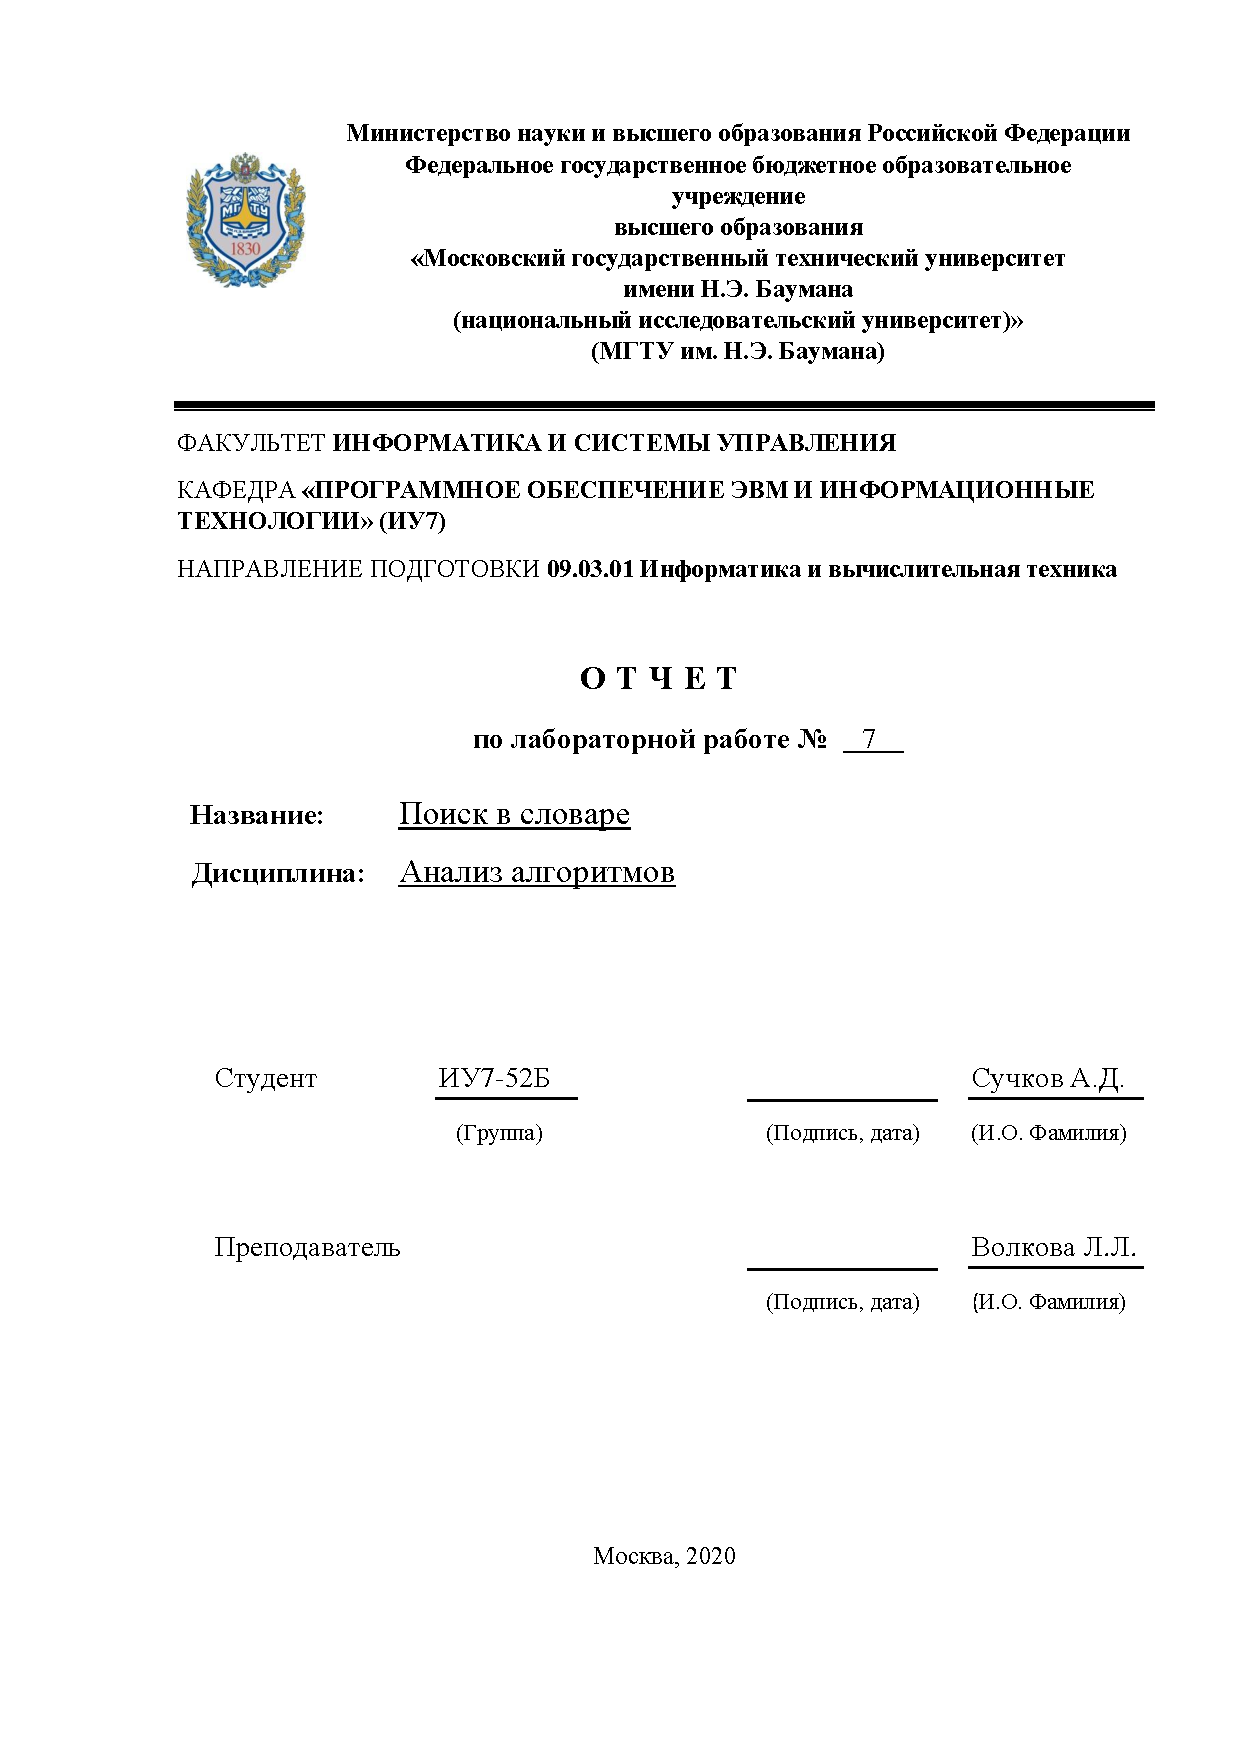
\includepdf[pages=1]{titul.pdf}
% Оглавление
\tableofcontents

\newpage
\chapter*{Введение}
\addcontentsline{toc}{chapter}{Введение}

В данной лабораторной работе реализуются и оцениваются алгоритмы поиска элемента в массиве словарей по ключу,
такие как алгоритм перебора, алгоритм бинарного поиска и сегментный поиск с частным анализом данных.

Поиск -- это операция при котором производится обработка некоторого множества данных с целью выявления 
подмножества данных, которые соответствуют критериям поиска. 

Словарь -- абстрактный тип данных, который позволяет хранить пары вида "(ключ значение)" и поддерживающий операции 
добавления пары, а также поиска и удаления пары по ключу. 

Поддержка словарей существует во многих интерпретируемых языках программирования высокого уровня, таких как Python, 
JavaScript, Ruby и других.

\newpage
\chapter{Аналитическая часть}

Целью лабораторной работы является разработка и исследование алгоритмов поиска элемента в массиве словарей.\\

Можно выделить следующие задачи лабораторной работы:
\begin{itemize}
    \item описание и реализация трёх алгоритмов поиска: алгоритм перебора, бинарного поиска и сегментного 
    поиска с частным анализом данных;
    \item проведение замеров процессорного времени работы алгоритмов;
    \item анализ полученных результатов.
\end{itemize}

\section{Поиск полным перебором}

Идея алгоритма заключается в том, что поиск заданного элемента из множества происходит непосредственно 
сравниванием каждого элемента этого множества с искомым, до тех пор, пока искомый не найдётся или множество
не закончится. 

Сложность алгоритма линейно зависит от объёма словаря, а время может стремиться к экспоненциальному времени 
работы.  

\section{Двоичный поиск в упорядоченном словаре}

Данный алгоритм содержит в себе идею, которая заключается в том, что берётся значение ключа из середины словаря и 
сравнивается с данным. 
Если значение меньше (в контексте типа данных) данного, то продолжается поиск в левой части словаря, при обратном случае - в правой. 
На новом интервале также берётся значение ключа из середины и сравнивается с данным. 
Так продолжается до тех пор, пока найденное значение ключа не будет равно данному\cite{analyse_info}.

Поиск в словаре с использованием данного алгоритма в худшем случае будет иметь трудоёмкость $O(log_{2}N)$, что быстрее 
поиска при помощи алгоритма полного перебора. 
Но стоит учитывать, что алгоритм бинарного поиска работает только для заранее отсортированного словаря. 

В случае большого объёма словаря и обратного порядка сортировки, может произойти так, что алгоритм полного перебора 
будет эффективнее по времени.  

\section{Сегментный поиск с частным анализом}

Идея алгоритма заключается в составлении частотного анализа. Чтобы провести частотный анализ, необходимо взять
первый элемент каждого значения в словаре по ключу и подсчитать частотную характеристику, т.е. сколько раз этот 
элемент встречается в качестве первого элемента. По полученным значениям словарь разбивается на сегменты так, 
что все элементы с одинаковым первым элементом оказываются в одном сегменте.

Далее сегменты упорядочиваются по значению частотной характеристики таким образом, чтобы элементы с наибольшей 
частотной характеристикой был самый быстрый доступ.

Далее каждый сегмент упорядочивается по значению. Это необходимо для реализации бинарного поиска, который 
обеспечит эффективный поиск в сегменте при сложности $O(N log N)$.

\section{Описание словаря}

В данной работе словарь представляет собой базу данных имён и имеет вид \{key: number, name: string\}. Поиск 
будет реализован по полю key.

\section{Вывод}

Результатом аналитического раздела стало определение цели и задач работы, описание используемых алгоритмов и 
описание самого словаря на котором будет проводится анализ.

\newpage
\chapter{Конструкторская часть}

В данном разделе представлены схемы рассматриваемых алгоритмов и требования к программному 
обеспечению.

\section{Схемы алгоритмов}

На рисунках 2.1 - 2.3 представлены схемы вышеописанных алгоритмов поиска в словаре.

\begin{figure}[h]
    \center{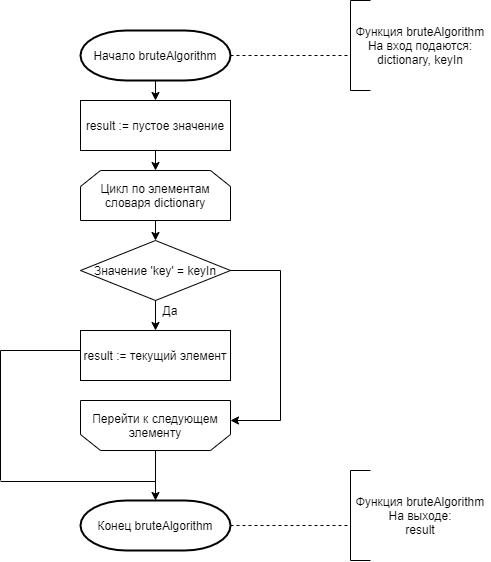
\includegraphics[scale=1]{sceheme_brute.png}}
    \caption{схема алгоритма поиска перебором}
    \label{fig:image}
\end{figure}

\begin{figure}[h]
    \center{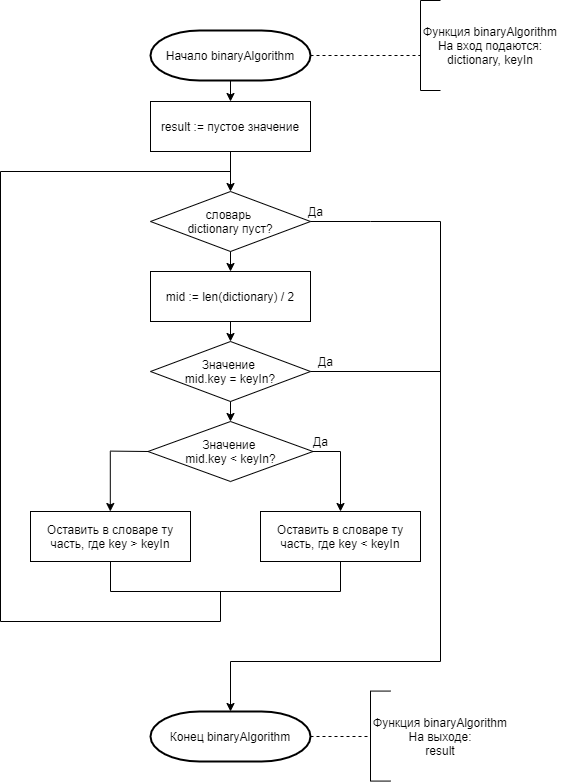
\includegraphics[scale=0.8]{sceheme_binary.png}}
    \caption{схема алгоритма бинарного поиска}
    \label{fig:image}
\end{figure}

\begin{figure}[h]
    \center{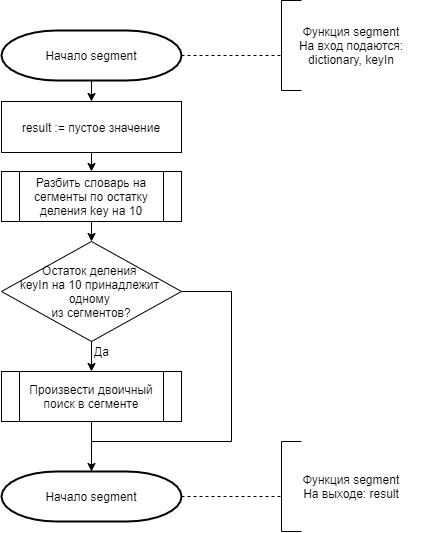
\includegraphics[scale=1]{scheme_segment.png}}
    \caption{схема алгоритма сегментного поиск с частным анализом}
    \label{fig:image}
\end{figure}

\section{Требования к программному обеспечению}

Для полноценного анализа и тестирования рассматриваемых алгоритмов необходимо обеспечить 
ряд требований:
\begin{itemize}
    \item предоставить выбор алгоритма для поиска и обеспечить консольный ввод ключа, 
    по которому будет происходить поиск;
    \item реализовать функцию замера процессорного времени, затраченного функциями.
\end{itemize}

\section{Вывод}

Результатом конструкторской части стало схематическое описание алгоритмов поиска в словаре и 
описание требований к программному обеспечению.

\newpage
\chapter{Технологическая часть} 

В данном разделе приведены средства для реализации рассматриваемых алгоритмов поиска, а также 
листинги кода.

\section{Выбор языка программирования}

В качестве языка программирования было решено выбрать Python 3, так как имеется опыт работы с библиотеками и 
инструментами языка, которые позволяют реализовать и провести исследования над алгоритмами поиска в словаре.

\section{Реализация алгоритмов}

В листингах 3.1 - 3.3 приведены реализации алгоритмов поиска в словаре.

\textrm{Листинг 3.1: функция поиска перебором}
\begin{lstlisting}[frame=single, numbers=left]
def bruteAlgorithm(dictionary, key):
    for item in dictionary:
        if item['key'] == key:
            return item

    return None
\end{lstlisting}

\textrm{Листинг 3.2: функция бинарного поиска}
\begin{lstlisting}[frame=single, numbers=left]
def binaryAlgorithm(dictionary, key):
    minE = 0
    maxE = len(dictionary) - 1
    midE = (minE + maxE) // 2

    tmp = dictionary[midE]['key']

    while key != tmp:
        if key < tmp:
            maxE = midE
        else:
            minE = midE

        midE = (minE + maxE) // 2
        tmp = dictionary[midE]['key']

    return dictionary[midE]
\end{lstlisting}

\textrm{Листинг 3.3: функции для организации сегментного поиска}
\begin{lstlisting}[frame=single, numbers=left]
def prepareSegment(dictionary, chance):
    chance = [[] for i in range(10)]

    for i in range(len(dictionary)):
        chance[dictionary[i]['key'] % 10]
        .append(dictionary[i])
    
    return chance


def segment(chance, key):
    segment = chance[key % 10]
    return binaryAlgorithm(segment, key)
\end{lstlisting}

\section{Оценка времени}

Для анализа времени алгоритмов поиска в словаре, реализована специальная функция, использующая 
библиотеку time \cite{time_bib}, листинг 3.4. \\

\textrm{Листинг 3.4: функция для замера процессорного времени работы}
\begin{lstlisting}[frame=single, numbers=left]
def doTimeTest():
    dictionary = []
    chance = []
 
    length = 100000
    repeat = 10000

    dictionary = fill(dictionary, length)
    chance = prepareSegment(dictionary)


    t1 = process_time()
    for i in range(repeat):
        bruteAlgorithm(dictionary, i)
    t2 = process_time()

    print("Time for brute -\t", (t2 - t1) / repeat)


    t1 = process_time()
    for i in range(repeat):
        binaryAlgorithm(dictionary, i)
    t2 = process_time()

    print("Time for binary -\t", (t2 - t1) / repeat)


    t1 = process_time()
    for i in range(repeat):
        segment(chance, i)
    t2 = process_time()

    print("Time for segment -\t", (t2 - t1) / repeat)
\end{lstlisting}

\newpage
\section{Результаты тестирования}

На рисунке 3.1 представлен скриншот интерфейса программы и тесты проведённые вручную.

\begin{figure}[h!]
    \center{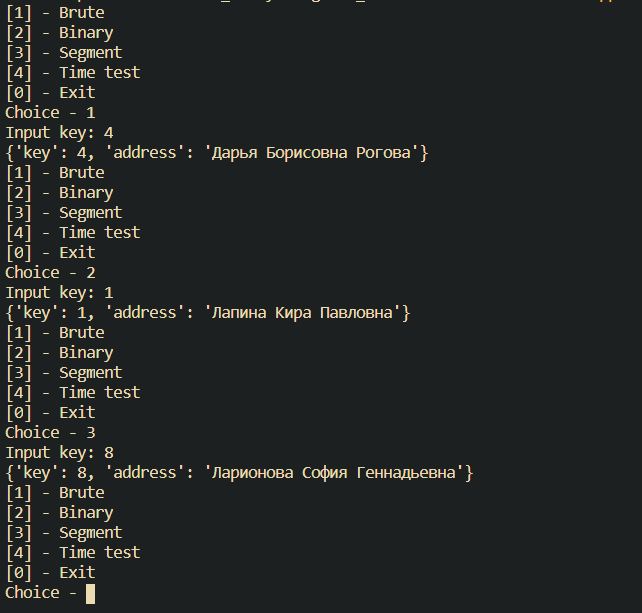
\includegraphics[scale=1]{tests.png}}
    \caption{схема алгоритма сегментного поиск с частным анализом}
    \label{fig:image}
\end{figure}

Все тесты прошли успешно.

\section{Вывод}

Результатом технологической части стал выбор используемых технических средств реализации 
и последующая реализация алгоритмов и замера времени работы на языке Python 3.

\newpage
\chapter{Исследовательская часть}

Измерения процессорного времени проводятся на размерах словаря 100, 1000, 10000 и 100000. 
Содержание словаря сгенерировано случайным образом с помощью библиотеки faker.

Для повышения точности, каждый замер производится 100000 раз, за конечный результат берётся 
среднее арифметическое.

\section{Результаты экспериментов}

Эксперименты проводились на компьютере со следующими характеристиками:
\begin{itemize}
    \item ОС - Windows 10, 64bit;
    \item Процессор - Intel Core i5 7300HQ 2.5GHz, 4 Core 8 Logical Processor
    \item ОЗУ - 8Gb
\end{itemize}

По результатом измерений процессорного времени можно составить таблицы 

\begin{table}[h!]
\caption{результаты проведённого заявками времени в очередях и системе}
\label{tabular:timesandtenses}
\begin{center}
\begin{tabular}{ | l | l | l | l | l | }
\hline
                     & 100                   & 1000                  & 10000                 & 100000                \\ \hline
    Поиск перебором  & $6.094 \cdot 10^{-6}$ & $5.813 \cdot 10^{-5}$ & $5 \cdot 10^{-4}$     & $3.495 \cdot 10^{-3}$ \\ \hline
    Бинарный поиск   & $4.688 \cdot 10^{-7}$ & $7.813 \cdot 10^{-7}$ & $1.250 \cdot 10^{-6}$ & $6.718 \cdot 10^{-6}$ \\ \hline
    Сегментный поиск & $9.375 \cdot 10^{-7}$ & $9.375 \cdot 10^{-7}$ & $1.406 \cdot 10^{-6}$ & $5.156 \cdot 10^{-6}$ \\ \hline
\end{tabular}
\end{center}
\end{table}

\section{Вывод}

Анализируя полученные результаты, можно сделать вывод, что алгоритм поиска в словаре, использующий поиск 
по сегментам с частотным анализом, выигрывает по скорости у алгоритма полного перебора и бинарного поиска, 
а в ряде случаев проигрывает.

Связано это с тем, что для алгоритма сегментного поиска необходимо провести частотный анализ, а уже после 
проводить поиск по сегментам. 
В том случае, когда искомый элемент находится в начале словаря, алгоритм полного перебора будет выигрывать 
как у алгоритма двоичного поиска, так и у алгоритма частотного анализа.

По таблице видно, что бинарный поиск и поиск по сегментам имеют практически схожие результаты, но стоит 
учитывать, что в итоговое время не было включено время сортировки словаря для алгоритма бинарного поиска.
Из этого можно заключить, что алгоритм поиска по сегментам будет работать быстрее.

\newpage
\chapter*{Заключение}
\addcontentsline{toc}{chapter}{Заключение}

В ходе выполнения лабораторной работы достигнута поставленная цель: разработка и исследование алгоритмов 
поиска по словарю. Решены все задачи.

Были изучены и описаны понятия словаря и поиска по словарю. 
Также были описаны и реализованы поиск полным перебором, бинарный поиск и сегментный поиск с частотным 
анализом.
Проведены замеры процессорного времени работы алгоритмов при различных размерах словаря. 
На основе экспериментов проведён сравнительный анализ.

Из проведённых экспериментов было выявлено, что бинарный поиск и поиск по сегментам имеют похожие 
результаты, но стоит учитывать, что в итоговое время не было включено время сортировки словаря для 
алгоритма бинарного поиска, поэтому можно предположить, что алгоритм поиска по сегментам с частотным 
анализом будет работать быстрее.

\newpage
\renewcommand\bibname{Список литературы}
\addcontentsline{toc}{chapter}{Список литературы}
\makeatletter % список литературы
\def\@biblabel#1{#1. }
\makeatother
\begin{thebibliography}{2}
    \bibitem{analyse_info} Дж. Макконнел. Анализ алгоритмов. Активный обучающий подход. -- М.: Техносфера, 2017. -- 267с.
    \bibitem{time_bib} Документация на официальном сайте Python про библиотеку time [Электронный ресурс]. Режим доступа: https://docs.python.org/3/library/time.html (дата обращения 23.09.2020)
\end{thebibliography}

\end{document}

